\clearpage
\section{Remote Robot Control: Desktop Implementation}
\label{sec:remote-control}
\textbf{Status: C++17 implementation, started by \texttt{onDesktop/runOperator}.} Teensy firmware revision 16 owns the acquisition timer; no automatic startup service is installed. The operator receives three ADC readings and returns motor commands through the ASUS Wi-Fi path. It reuses the local line-following decision rules at 100 sensor triplets/s. The timing numbers later in this section were recorded with motor output disabled.

\subsection{Programs and Responsibilities}
The source is one tree, \path{lineFollowerDistributed/}, compiled on the Pi and on the Desktop. The Pi entry point is \texttt{controller}; the Desktop entry point is \texttt{run\_operator}, started by \texttt{onDesktop/runOperator}. The two binaries default to motor-disabled operation. \texttt{runOperator} passes \texttt{--enable-motors} to both unless \texttt{--disable-motors} is given, in which case the Pi writes \texttt{STOPALL} and the wheels stay stopped. The same duration is given to both programs and starts after the job handshake. The default speed is 0.5.

The Pi controller owns the UART, motor polarity (default \texttt{rr}), limits, session handling and the stop policy. The Desktop operator owns calibration use and the line-following decision. It does not keep a calibration file of its own. At job start the controller reads three JSON files on the Pi and sends their bytes in one UDP datagram. A C++17 compiler and Make build the programs natively on Pi and macOS. The control programs have no Python dependency. JSON and SHA-256 headers are vendored with their licenses; Teensy requires firmware revision 16.

\begin{table}[H]
\centering\small
\caption{Implemented division of the current program.}
\label{tab:remote-split}
\begin{tabular}{@{}L{3.0cm}L{6.2cm}L{7.0cm}@{}}
\toprule
Responsibility & Pi: Controller & Desktop: Operator \\
\midrule
Sensor acquisition & Own UART exclusively; receive timer-driven Teensy samples; validate counts and forward timestamps. & Receive readings; use the newest valid sample for the next decision. \\
Line following & No tape detection or steering calculation. & Calibration, \texttt{SigmaDeadband}, \texttt{tape\_seen}, \texttt{normalize}, \texttt{gradient\_noise}, \texttt{motor\_targets}. \\
Motor execution & Validate targets; apply wiring polarity once; send MOTORS/STOPALL; track acknowledgement. & Return signed physical left/right PWM values together, including unchanged targets while active. \\
Lifetime and status & Enforce session, sequence, sample-age limit, local run limit and stop policy. & Accept the initialization datagram, then start, arm and stop the session. Identify the sensor file by the hash of the received bytes. Report transmit latency and its uncertainty. \\
\bottomrule
\end{tabular}
\end{table}

The Pi remote process owns UART exclusively; no other serial client may run concurrently. The three JSON files stay on the Pi. The operator receives their bytes over UDP and does not read them from a shared disk. Desktop sends physical signed targets in $[-255,255]$, not raw direction-pin settings. These represent direction and PWM magnitude, not measured wheel speed.

\texttt{runOperator} refuses any Pi address other than Wi-Fi \texttt{10.0.0.20}. It prints the effective arguments, checks the plant, and starts the controller over SSH. The controller binds the addresses of that SSH connection and waits. The operator then uses Pi port 5000 and Desktop port 5001; the Desktop address is the one reported by the controller, \texttt{10.0.0.2} when the Desktop Ethernet is on the ASUS. SSH starts and stops the controller. It does not copy \path{boot.json}, \path{clock_calib.json} or \path{photo3_calib.json}.

\subsection{Initialization Datagram}
\label{sec:init-datagram}
When the controller accepts a job request it reads \texttt{/proc/uptime} and three files in \path{/home/pi/plant_lineFollower/config/}. \path{photo3_calib.json} is required. \path{boot.json} and \path{clock_calib.json} are included when present and are empty sections when absent. One UDP datagram carries all three. It is not one of the 128-byte control frames. Its 27-byte header is the six characters \texttt{LFINIT}, version 1, Pi uptime in milliseconds as a big-endian 64-bit integer, and the three file lengths as big-endian 32-bit integers. The raw file bytes follow, in the order boot, clock, then photo. Each file is at most 20\,000 bytes. The controller sends the same datagram again with every job-ready retry. The operator accepts that datagram and the job-ready frame in either order, writes the three files into the run log, and only then builds the decision and the clock report.

From \path{photo3_calib.json} the operator reads only the white and black mean and standard deviation of sensors A, B and C. It treats those means as usable and does not consult the file's validity flag. It does not take motor polarity from the file; polarity remains the controller setting, default \texttt{rr}. The SHA-256 of the received photo bytes is the calibration identity in the following HELLO, so both sides agree on the same bytes before arming.

\path{boot.json} carries \texttt{hash8}, the Pi local time and \texttt{uptime\_s} written at boot. \path{clock_calib.json} is the summary from Appendix~\ref{sec:gpio-clock}. The operator uses that summary only when its \texttt{hash8} equals the boot file, the Pi--Teensy half completed, and at least one Wi-Fi probe was valid. Elapsed time $\Delta t$, in seconds, is the uptime in the datagram minus \texttt{uptime\_s} in the clock file. With $w$ the median Wi-Fi half-width in milliseconds, $r$ the detrended residual range in microseconds and $b$ the fitted drift in ppm,
\begin{equation}
u = w + \frac{r}{1000} + |b|\,\Delta t \times 10^{-3}
\qquad[\mathrm{ms}].
\label{eq:transmit-uncertainty}
\end{equation}
The Ethernet half-width is not used on a robot run. The Wi-Fi midpoint and the nominal Pi$-$Teensy offset convert the Teensy sample-complete time into Desktop time. Transmit latency is Desktop receipt of the SENSOR datagram minus that instant. The midpoint is a clock origin, not a delay. If the hashes differ, either file is missing, or the summary is incomplete, each sample instead contributes the raw delivery upper bound already in the SENSOR frame: Pi completion time minus the conservative earliest bound. The median of those bounds is then reported as the uncertainty. A Teensy-only reset does not change \texttt{hash8}.

A 10\,s motor-enabled run on October 11 used the summary in Section~\ref{sec:clock-delay-current}. The initialization datagram carried \texttt{hash8} \texttt{f03276bd} for both files, so the clocks matched. Pi uptime in that datagram was 2592.47\,s, 390.5\,s after the clock file. Equation~\eqref{eq:transmit-uncertainty} was then $1.036+0.038+1.070=2.143$\,ms: most of the uncertainty is drift since the calibration, not the Wi-Fi half-width. The operator received 998 sensor packets with no sequence gaps and sent 989 commands. Transmit latency had median 3.947\,ms, 99th percentile 12.096\,ms and maximum 20.195\,ms, each with that 2.143\,ms uncertainty. Desktop computation had median 0.001\,ms. On the Pi, 999 triplets were acquired and all 998 successive start intervals were 10\,ms. It accepted 989 commands, acknowledged 974, replaced 15 that were still waiting, and made 974 nonzero motor writes. Teensy standby was confirmed on the Pi. The Desktop log is \path{lineFollowerDistributedBin/out/20261011_115032_cpp_operator_43586/}; the Pi log is \path{lineFollowerDistributedBin/out/20261011_111348_cpp_controller_1879/}. The Pi wall clock lags the Desktop, which is why those directory times differ.

\begin{figure}[H]
\centering
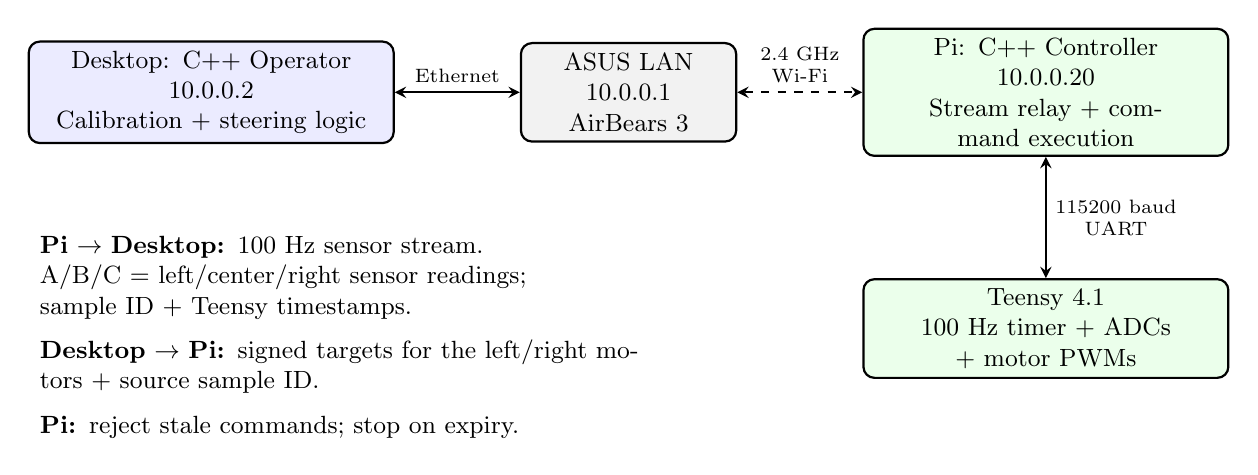
\begin{tikzpicture}[font=\small,>=stealth,
 block/.style={draw,thick,rounded corners,align=center,text width=4.4cm,minimum height=1.25cm},
 link/.style={<->,thick}, note/.style={font=\scriptsize,align=center,fill=white,inner sep=3pt}]
\node[block,fill=blue!8] (desktop) at (0,0) {Desktop: C++ Operator\\10.0.0.2\\Calibration + steering logic};
\node[block,fill=gray!10,text width=2.5cm] (asus) at (5.3,0) {ASUS LAN\\10.0.0.1\\AirBears 3};
\node[block,fill=green!8] (pi) at (10.6,0) {Pi: C++ Controller\\10.0.0.20\\Stream relay + command execution};
\node[block,fill=green!8] (teensy) at (10.6,-3.0) {Teensy 4.1\\100 Hz timer + ADCs + motor PWMs};
\draw[link] (desktop) -- node[note,above] {Ethernet} (asus);
\draw[link,dashed] (asus) -- node[note,above] {2.4 GHz\\Wi-Fi} (pi);
\draw[link] (pi) -- node[note,right] {115200 baud\\UART} (teensy);
\node[align=left,text width=7.9cm,anchor=north west] at (-2.3,-1.7) {\textbf{Pi $\to$ Desktop:} 100 Hz sensor stream.\\A/B/C = left/center/right sensor readings;\\sample ID + Teensy timestamps.\\[5pt]\textbf{Desktop $\to$ Pi:} signed targets for the left/right motors + source sample ID.\\[5pt]\textbf{Pi:} reject stale commands; stop on expiry.};
\end{tikzpicture}

\caption{Implemented remote split on the configured network. Teensy owns acquisition timing and motor PWM; Pi relays samples and validates commands; every line-following decision is made on the Desktop. ASUS only transports packets, including the initialization datagram. A run with \texttt{--disable-motors} replaces proposed targets with STOPALL at the Pi UART boundary; otherwise the Pi applies the signed targets.}
\label{fig:remote-topology}
\end{figure}

\clearpage
\subsection{Independent Sampling and Immediate Decisions}
Teensy is the sampling-clock master. Its PIT hardware timer (\texttt{IntervalTimer}) invokes acquisition every 10\,ms at the default 100\,Hz. The interrupt handler reads A/B/C sequentially, records start and completion in Teensy microseconds, and puts the triplet in a fixed ring. Each conversion has a 100\,$\mu$s timeout. There is no UART formatting or transmission inside the interrupt. A conversion fault drives STBY low to disable the motors and ends the stream. The timer uses a peripheral separate from the motor PWM timers.

The firmware main loop sends complete sample lines when UART transmit space is available, while handling motor commands and watchdogs. Its 16-slot ring holds at most 15 pending triplets; overflow drops a new sample and increments a counter. Sequence gaps expose missing data, and the original timestamps expose buffering. The three readings are sequential conversions, not simultaneous ADC captures. Hardware-timer interrupts still have finite latency; timing stability is measured, not assumed.

Pi sends \texttt{STREAM 100} once, then consumes unsolicited samples. It does not issue periodic \texttt{ADC3} requests or pace sampling with Linux sleeps. One C++ event loop handles nonblocking UART and UDP, with a parser that separates sample lines from command acknowledgements. Only one command reply is outstanding, but any number of sample lines may arrive between replies. The Pi periodically queries \texttt{CLOCK} to relate Teensy time to Pi time; this query does not trigger acquisition. Stop takes priority over ordinary commands. A missing stream, invalid timestamp/sequence, UART timeout or parser failure stops the controller. The stream timeout is the larger of 80\,ms and three sample periods.

Packet buffers, a 512-entry sample history, pending targets and telemetry rings have fixed capacities. JSON parsing, calibration hashing and log-file writing remain outside the control loop. The UART writer checks target expiry again before transmitting pending motor bytes. Normal exit sends \texttt{STOPALL}, ends streaming and verifies standby. No boot service is installed.

Desktop is event driven. It receives a valid sensor packet, performs the existing calibrated calculation and sends both wheel targets immediately, without a separate 100\,Hz sleep. If readings accumulated while it was busy, it drains the bounded input buffer and computes from the newest reading, recording skipped samples. The deadband then evolves on the processed samples; after drops this is not identical to processing every sample in the original loop. Replay comparisons therefore use identical processed sample sequences.

\begin{figure}[H]
\centering
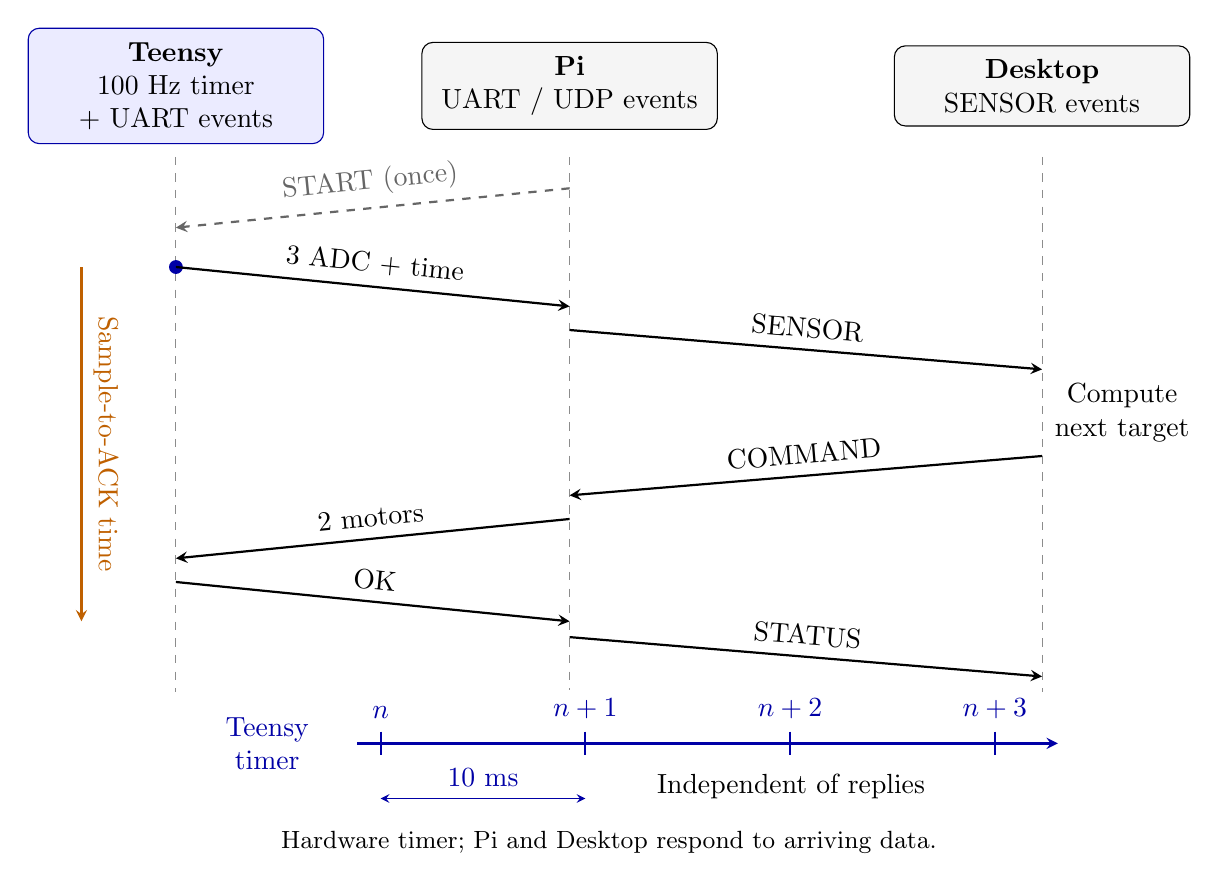
\begin{tikzpicture}[font=\normalsize,>=stealth,
 note/.style={font=\normalsize,fill=white,align=center,inner sep=3pt},
 arrowlabel/.style={font=\normalsize,sloped,above=3pt,inner sep=1pt},
 device/.style={draw,rounded corners,align=center,text width=3.4cm,inner sep=5pt},
 msg/.style={->,thick}]
\node[device,draw=blue!65!black,fill=blue!8] at (0,.5) {\textbf{Teensy}\\100 Hz timer\\+ UART events};
\node[device,fill=gray!8] at (5,.5) {\textbf{Pi}\\UART / UDP events};
\node[device,fill=gray!8] at (11,.5) {\textbf{Desktop}\\SENSOR events};
\foreach \x in {0,5,11} \draw[dashed,black!45] (\x,-.4) -- (\x,-7.2);
\fill[blue!65!black] (0,-1.8) circle (2.5pt);
\draw[msg,dashed,black!60] (5,-.8) -- node[arrowlabel] {START (once)} (0,-1.3);
\draw[msg] (0,-1.8) -- node[arrowlabel] {3 ADC + time} (5,-2.3);
\draw[msg] (5,-2.6) -- node[arrowlabel] {SENSOR} (11,-3.1);
\node[note,anchor=west] at (11.05,-3.65) {Compute\\next target};
\draw[msg] (11,-4.2) -- node[arrowlabel] {COMMAND} (5,-4.7);
\draw[msg] (5,-5.0) -- node[arrowlabel] {2 motors} (0,-5.5);
\draw[msg] (0,-5.8) -- node[arrowlabel] {OK} (5,-6.3);
\draw[msg] (5,-6.5) -- node[arrowlabel] {STATUS} (11,-7.0);
\draw[->,thick,orange!75!black] (-1.2,-1.8) -- node[arrowlabel] {Sample-to-ACK time} (-1.2,-6.3);
\node[note,text=blue!65!black,anchor=east] at (1.8,-7.85) {Teensy\\timer};
\draw[->,thick,blue!65!black] (2.3,-7.85) -- (11.2,-7.85);
\foreach \x/\n in {2.6/n,5.2/{n+1},7.8/{n+2},10.4/{n+3}} {
  \draw[thick,blue!65!black] (\x,-7.7) -- (\x,-8.0);
  \node[note,above,text=blue!65!black] at (\x,-7.65) {$\n$};
}
\draw[<->,blue!65!black] (2.6,-8.55) -- node[arrowlabel] {10 ms} (5.2,-8.55);
\node[note,anchor=west] at (6,-8.4) {Independent of replies};
\node[note,font=\small,anchor=north] at (5.5,-8.85) {Hardware timer; Pi and Desktop respond to arriving data.};
\end{tikzpicture}

\caption{Teensy samples every 10\,ms from its hardware timer (blue). Pi responds to UART/UDP arrivals; Desktop computes on SENSOR arrival. START is sent once per controller launch. The bottom timer runs independently of replies; the sample-to-ack interval is reported as a clock-mapping upper bound. Message-sequence spacing is schematic, not a latency scale.}
\label{fig:remote-timing}
\end{figure}

\subsection{Transport and Version 2 Message Contract}
Control traffic is direct binary UDP on the ASUS LAN. \texttt{runOperator} uses Pi \texttt{10.0.0.20:5000} and the Desktop address reported by the controller, port 5001. The operator runs natively on macOS, without a container or VM. Only one active operator session controls the robot. The initialization datagram in Section~\ref{sec:init-datagram} uses this same socket and is not an SSH or \texttt{scp} transfer.

\begin{table}[H]
\centering\small
\caption{Implemented version 2 message contents. Exact big-endian struct layouts and golden-frame tests are included in each package.}
\label{tab:remote-messages}
\begin{tabular}{@{}L{3.3cm}L{12.9cm}@{}}
\toprule
Packet & Required information \\
\midrule
Common header & Magic, protocol version, message type, payload length, session ID and sequence number; explicit network byte order and fixed-width fields. \\
SENSOR: Pi to Desktop & Sample ID; Teensy start/end timestamps (microseconds); A/B/C uint16 counts; missing-sample count; conservative Pi completion bound and Pi receipt time (nanoseconds); original Teensy sequence. \\
COMMAND: Desktop to Pi & Command ID; source sample ID; signed left/right int16 PWM targets ($-255\ldots255$). Session and sample identity link the decision to its original observation. \\
STATUS: Pi to Desktop & Last command acknowledged by Teensy; source sample ID; Pi send/ack timestamps; armed/stopped/fault state and rejection/loss counters. Acknowledgement is not proof of motor rotation. \\
Initialization & One datagram, magic \texttt{LFINIT}: Pi uptime and the raw bytes of \path{boot.json}, \path{clock_calib.json} and \path{photo3_calib.json}. Sent with each job-ready reply, before HELLO. \\
Session control & HELLO/configuration agreement, ARM, STOP and acknowledgements. Agree rate, freshness limit, maximum PWM, run duration, motor enable, polarity and the SHA-256 of the received sensor file before arming. \\
\bottomrule
\end{tabular}
\end{table}

At 100\,Hz the three raw uint16 values are 600\,bytes/s before headers. Version 2 uses a 24-byte application header, an 82-byte SENSOR frame and a 36-byte COMMAND frame: 11.8\,kB/s combined at 100 messages/s in each direction. These frame lengths are UDP payload sizes, excluding UDP/IP headers. STATUS is 75 bytes, sent after each UART command acknowledgement and periodically. Session traffic and UDP/IP/Wi-Fi overhead are additional. SENSOR, COMMAND, STATUS and the session-control frames do not exceed 128 bytes. The initialization datagram is separate and larger: the three current summaries are a few kilobytes, and each included file is limited to 20\,000 bytes. Section~\ref{sec:message-sizes} separates binary LAN payloads from ASCII UART record lengths and compares the stale 25, 50 and 100\,Hz runs. Larger steady-state payloads must use an explicit size/rate budget, avoid IP fragmentation, and include pacing and overload handling; they cannot simply expand without limit.

UDP preserves message boundaries but does not guarantee delivery or order. Drop duplicate, reordered and expired control data; do not retransmit obsolete samples or drive commands. Lost data is exposed by sequence gaps. Session-control exchanges use bounded retries and idempotent acknowledgements; repeated STOP is harmless. A fresh session ID prevents packets from a previous run from taking control. Pin the active peer address/port; the session ID distinguishes runs and is not cryptographic authentication. This protocol is intended for the isolated robot LAN, not direct Internet exposure. These choices follow the \href{https://www.rfc-editor.org/rfc/rfc8085.html}{UDP usage guidelines}.

\subsection{Freshness, Stop Behavior and Recovery}
The installed default freshness limit is \textbf{100\,ms}. Each run records its actual limit; acquisition remains 100\,Hz. Pi retains a fixed-size ring from recent sample IDs to conservative completion-time bounds on its own clock. A \texttt{CLOCK} query establishes that the Teensy-reported instant occurred after Pi sent the query. Mapping allows 1,000\,ppm relative oscillator error and 2\,$\mu$s timestamp quantization; the mapping is refreshed every second and expires after two seconds. This is a documented drift assumption, not synchronized wall clocks. Buffering before Pi receives a sample consumes its lifetime instead of resetting it. At reception and immediately before serial transmission, it rejects commands referencing unknown or expired samples, invalid ranges, older command IDs or the wrong session. Thus no synchronized Desktop/Pi clocks are required for command-age checks.

A valid command expires at its source sample's conservative completion bound plus the freshness limit, not a new full lifetime after a delayed network arrival. Repeated or duplicate packets cannot extend this deadline. Both motors stop when the active command expires, on explicit STOP, local run-time expiry, sensor/serial failure, or process shutdown when communication is still available. An invalid packet never refreshes drive lifetime. Desktop loss therefore stops the robot even if Pi and Teensy remain running. Stop dispatch and UART acknowledgement add measurable delay; the freshness limit is a software policy, not a guaranteed physical stopping time.

Start stopped. Require explicit arming with a fresh session and valid recent sensor exchange. After a communication timeout/fault, remain stopped until explicitly rearmed; delayed packets must not restart motion. Normal tape loss is different: Desktop sends fresh zero targets while the session remains active, allowing the original tape-reacquisition behavior within the run limit. Pi retains a local maximum PWM and duration limit even though Desktop chooses the steering.

The existing Teensy firmware watchdog stops drive after approximately 750\,ms without a valid drive refresh. It is backup for a hung Pi process, not the configured network freshness policy. Pi must never continually refresh a command after its source sample expires. Revision 10 preserves this independent motor watchdog; sampling and clock queries do not refresh it. Tests verify serial replies and stopped status; the firmware watchdog under real motion and physical stopping distance remain untested.

\subsection{Timing Measurements and Demonstration Sequence}
Current telemetry video is Appendix~\ref{app:telemetry-video}. The September recordings use the stale per-job GPIO-plus-network alignment and sample-to-target-receipt timing defined in Section~\ref{sec:desktop-clock}. A current \texttt{runOperator} session does not repeat that calibration; it reports the transmit latency of Section~\ref{sec:init-datagram}. The sample-to-ACK upper bound below is an earlier diagnostic with different endpoints; it must not be compared directly with that transmit latency.

Measure actual acquisition intervals, missed ticks, command age, UDP sequence gaps, queue drops, Pi CPU load and Desktop compute duration. Report median, 99th/99.9th percentile, maximum observed delay and the longest interruption, with run duration and sample count. Keep per-packet logging out of the critical path; use bounded buffering and summarized console output.

Acquisition duration and sample intervals use Teensy's own microsecond timestamps. Delivery age and sample-to-ack latency use a conservative mapping to Pi monotonic time:
\begin{equation}
T_{\mathrm{sample\ to\ ack}}^{\mathrm{upper}}=t_{\mathrm{Teensy\ ack,Pi}}-t_{\mathrm{sample\ completion,Pi}}^{\mathrm{lower}}.
\end{equation}
This bound includes sample forwarding, Desktop computation, return transmission and UART acknowledgement. It includes clock-mapping uncertainty and is not directly equivalent to the historical Pi-receipt-to-ack metric below. Desktop reports its local compute duration without subtracting timestamps from different hosts. The firmware sends both ADC start and end; reported sample intervals on Pi use successive starts.

\begin{enumerate}
\item Replay recorded ADC sequences with the same calibration through the local reference and Desktop decision logic; compare signed motor targets, tape-loss behavior and deadband resets.
\item Run live sensors at 100\,Hz with motors disabled; exercise the full sensor/decision/return path, rejecting or replacing nonzero targets before UART drive. Report synthetic-response and actual UART-ack timing separately.
\item Inject loss, duplicates, reordering and delay; stop Desktop and interrupt Wi-Fi. Verify that stale data cannot extend motion or restart an expired session. Exercise bounded UART timeout paths.
\item With motor testing explicitly enabled, use raised wheels for a short low-PWM trial, verify directions and measured stop behavior, then conduct a short floor trial on tape.
\item Increase sample rate and payload size separately. Sampling already uses Teensy timestamps and a hardware timer. For higher rates, reassess ADC interrupt cost, UART bandwidth, framing and buffering; consider hardware ADC triggering/DMA.
\end{enumerate}

The first acceptance goal is a demonstrated loop with measured timing and stop behavior, not a hard real-time claim. Linux/macOS scheduling and network delivery still introduce jitter; a C++ port does not establish hard real-time guarantees. Neither working SSH nor sufficient average bandwidth demonstrates a sustainable 100\,Hz control loop. Appendix~\ref{app:long-term} holds the larger future workload and Appendix~\ref{sec:motion-control} preserves the simulation model for later comparisons.

\subsection{C++ Packages and Validation}
The measurements in this subsection used firmware revision 10. The firmware installed now is revision 16, and both C++ packages are built. The updated unit suite passed 3,100 checks on Pi and Desktop, including all 3,012 steering-reference decisions; virtual-UART tests also passed on both hosts (with AddressSanitizer/UndefinedBehaviorSanitizer on Mac).

A 15.01\,s Desktop session on the home-network comparison path received 1,500 triplets and sent 1,484 decisions. Pi collected 2,499 triplets over its 25\,s sampling run, with no missing sequence numbers. All reported Teensy start intervals were 10,000\,$\mu$s; ADC duration was about 53\,$\mu$s. The sample-to-ACK upper bound had median 10.37\,ms, 99th percentile 22.92\,ms and maximum 30.47\,ms. These are clock-mapping bounds, not directly comparable to the historical round-trip numbers below. STOP was acknowledged and standby confirmed.

In a separate five-second test, deliberately suspending Pi produced a 203.40\,ms loop gap. Teensy still reported 10,000\,$\mu$s intervals for all 499 received triplets, with no sequence gaps; the delivery-age bound reached 198.18\,ms. This demonstrates that Pi scheduling no longer sets acquisition timing. A live motor-disabled protocol probe also verified invalid/duplicate packet rejection, command-loss expiry, late-ARM rejection and confirmed STOP. No physical motor drive was enabled.

The ASUS link recovered after the adapter reset: the original script attempted activation just before NetworkManager declared the device ready, then automatic reconnection succeeded four seconds later. The recovery script now waits up to 30\,s for readiness and recognizes automatic reconnection. That test used Wi-Fi \texttt{10.0.0.20} on host \texttt{pi2}. A robot run still uses that Pi address; the Desktop address is the one the controller reports for the SSH session.

The subsequent ASUS test collected 7,499 triplets over 75.059\,s on Pi with zero sequence gaps and all reported start intervals at 10,000\,$\mu$s. Desktop received 5,016 triplets and sent 4,957 decisions, but the 100\,ms freshness policy stopped its session after 50.188\,s of the intended 60\,s. The longest command-arrival gap was 102.806\,ms while Pi's largest loop gap was only 5.689\,ms and Teensy sampling continued. This identifies a command-delivery delay; it does not distinguish Desktop scheduling from Wi-Fi delay. The acknowledged sample-to-ACK upper bound had median 9.215\,ms, 99th percentile 16.563\,ms and maximum 40.085\,ms. Motors stayed disabled, STOP was acknowledged, and final standby was confirmed. Default freshness remains 100\,ms; uninterrupted wireless operation at that limit is not yet established. Details are in \texttt{VALIDATION\_TEENSY\_CLOCK.md}.

\subsubsection{Earlier C++ Pi-Clock Baseline}
The measurements below predate Teensy-clock firmware and are preserved for comparison.

Each package includes a README, configuration, protocol documentation, dependency declaration and tests. Pi additionally includes the serial engine and independently tested command-lifetime policy. In this earlier package, Desktop carried the pure steering functions and a calibration snapshot copied from the Pi; source and calibration hashes were recorded in \texttt{provenance.json}, and updating calibration was an explicit paired copy. The current operator does not keep that snapshot. It receives the Pi files in the initialization datagram.

The native C++ tests passed on Pi and Desktop: 3,012 reference steering decisions matched, with 3,086 checks in the original unit executable (3,100 after the Teensy-clock changes). Virtual-UART integration tests verify motor-disabled output, polarity mapping with simulated motors, command-loss stopping, late ARM rejection, a missing sensor stream, partial/interleaved sample and acknowledgement lines, and expiry before UART transmission. Clock tests check stale-buffer handling, reset rejection and 64-bit timestamps across a 32-bit microsecond rollover. The same controller tests passed on macOS with AddressSanitizer and UndefinedBehaviorSanitizer. Those simulated tests never open the robot UART.

Current C++ reports use \texttt{events.csv} and \texttt{summary.json}. A 60,000-event ring and 30,000 observations per timing metric bound memory use. Reports include total counts, overwritten-event counts, retained-window percentiles and whole-run maxima. Logs are written after final stop. The two runtime entry points and all current automated tests are C++.

The first C++ ASUS protocol probe passed with proposed targets $+80/-40$ and zero applied PWM. It rejected invalid/duplicate packets, stopped on command loss, rejected late rearming and acknowledged STOP. A following strict run collected 7,499 triplets over 75.05\,s with one missed acquisition tick. Desktop's 100\,ms session expired after 30.74\,s, when the incoming-command gap reached 128.70\,ms. The Pi's largest loop gap was 19.59\,ms and largest ADC interval 24.91\,ms. The acknowledged round-trip median was 4.08\,ms and the 99th percentile 15.42\,ms. Pi continued sampling without a UART fault and confirmed standby on exit. A package-backup transfer overlapped the beginning of this run; it was not an isolated-load benchmark.

A separate C++ run with temporary 250\,ms freshness and the unchanged 80\,ms UART deadline completed the entire 60.007\,s Desktop session. Desktop received 5,999 sensor triplets and sent 5,930 decisions. Pi acquired exactly 7,500 triplets during its 75.051\,s process lifetime, with zero missed acquisition ticks. It acknowledged 5,909 commands and replaced 21 pending targets. Median acknowledged round trip was 3.88\,ms, the 99th percentile 12.69\,ms, and the maximum 42.81\,ms. The whole-run maximum Pi loop gap was 6.46\,ms; acquisition intervals had median 9.98\,ms, 99th percentile 11.26\,ms and maximum 14.20\,ms. Desktop computation had median 0.001\,ms and 99th percentile 0.002\,ms. Pi consumed 15.066 CPU seconds over its 75.051\,s lifetime (about 20\% of one core, including 15\,s of sampling after Desktop stopped).

Both programs exited normally, STOP was acknowledged, and final Teensy standby was confirmed. In all three live C++ runs, the UART audit contained only ADC3 and STOPALL, with zero nonzero motor writes and no audit overwrites. No motor motion was enabled. Defaults remain 100\,ms freshness and an 80\,ms serial deadline. Each package's \texttt{VALIDATION\_CPP.md} contains exact report paths, reproduction commands and limitations. These results do not establish reliable long-term operation through a wireless link at the stricter freshness limit.

\subsection{Why the Remote Implementation Moved from Python to C++}
The split Python prototype demonstrated the communication loop, but measurements on the current Pi motivated its replacement:
\begin{itemize}
\item \textbf{Garbage-collection pauses.} A measured 54.7\,ms collection coincided with a 57.2\,ms controller gap---almost six periods of the 100\,Hz sampling schedule then running on Pi.
\item \textbf{CPU overhead.} The Python diagnostic used about 82\% of one Pi core, compared with about 20\% in the later C++ run. These separate runs indicate substantially more processing headroom, rather than a controlled language benchmark.
\item \textbf{Control-loop latency.} In the diagnostic runs, median Pi-receipt-to-ack latency fell from about 15.7\,ms to 3.9\,ms with C++; fixed buffers and preallocated telemetry also make runtime work easier to bound.
\end{itemize}
C++ removes Python garbage collection, but it does not eliminate Linux scheduling or wireless delivery delays. Acquisition timing therefore moved to Teensy's hardware timer as a separate improvement. Desktop retains the same calibrated steering rules, verified against 3,012 reference decisions; a network freshness watchdog remains necessary.
